\documentclass[12pt,letterpaper]{article}

\usepackage[utf8]{inputenc}
\usepackage[T1]{fontenc}
\usepackage[spanish,es-noshorthands]{babel}
\usepackage{lmodern}
\usepackage{geometry}
\geometry{margin=2.5cm}
\usepackage{graphicx}
\usepackage{float}
\usepackage{hyperref}
\hypersetup{
  colorlinks=true,
  linkcolor=black,
  urlcolor=blue
}

\title{Base de datos musical}
\author{Jonathan}
\date{\today}

\begin{document}

\maketitle

\begin{abstract}
En este proyecto se realizó una base de datos musical con una interfaz
gráfica para el usuario. Al ejecutar el programa por primera vez, la
interfaz aparece vacía, y el usuario debe escoger una carpeta para
minarla: se buscan todos los archivos MP3 que contenga y, a partir de sus
etiquetas ID3v2.4, se llena la base de datos con la información de cada
canción, como su título, su intérprete, su álbum, su año y su género. Si
después se escoge otra carpeta, su contenido reemplaza al anterior. Al
terminar el minado se pueden ver las rolas con su información, y también
editar sus datos (título, intérprete, pista, año, género y álbum); estas
modificaciones se hacen siempre en la base de datos y nunca en los
archivos MP3. Además, el usuario puede definir si un intérprete es una
persona o un grupo, dar de alta personas nuevas aunque no tengan ninguna
canción, agregar miembros a los grupos y hacer búsquedas con un lenguaje
sencillo, sin necesidad de escribir SQL.
\end{abstract}

\tableofcontents

\section{Introducción}

Uno de los retos más difíciles de este proyecto fue hacer y entender la
interfaz gráfica, sobre todo por la herramienta que elegí, que sirve tanto
para Android como para computadora. Ya tenía algo de experiencia con
interfaces gráficas por el curso de ICC, donde usamos JavaFX con FXML, pero
esta forma de construirlas era muy distinta. Otra cosa muy nueva fue la
base de datos en SQL: en ICC ya había hecho una pequeña base de datos de
chocolates, a la que, la verdad, ni se le podría llamar base de datos
comparada con esta. Lo que más me confundió fue cómo conectar a cada
intérprete con su persona o su grupo, y cómo agregar varias personas como
miembros de un mismo grupo. El minero también fue complicado al principio,
por tener que leer cada etiqueta ID3, aunque poco a poco se volvió más
fácil.

Lo que más me costó fue el compilador del buscador, que toma lo que
escribe el usuario en un lenguaje sencillo y lo convierte en SQL. Para
lograrlo, primero se corta el texto en piezas, después se acomodan en un
árbol que conecta cada operador respetando su orden, y al final ese árbol
se recorre para formar la consulta que hace la búsqueda. También se
pusieron en práctica temas del curso, como el patrón Singleton, que se usó
para que todo el programa compartiera una sola conexión a la base de
datos, y el patrón Modelo-Vista-Controlador, que en este proyecto fue muy
efectivo porque deja muy claro en qué parte va cada cosa.

Este proyecto se parece mucho a aplicaciones como Spotify o Google Play
Música, que muestran el artista, el nombre de la canción y el álbum al que
pertenece. Se parece sobre todo a Play Música, porque ahí también había
que escoger la carpeta de donde se leían tus MP3, y a los artistas o
canciones que no tenían esa información les ponía ``Unknown''. Gracias a
este proyecto por fin entendí por qué me pasaba eso en esa época: los
archivos no traían esos datos en sus etiquetas. Además, ahí se podían
reproducir las canciones y hacer otras cosas con ellas, que es algo que me
gustaría agregarle a mi proyecto en el futuro, ya que lo seguiré
actualizando en mi tiempo libre.

Utilicé Kotlin porque ya estaba familiarizado con él, y así podía
concentrarme solamente en las cosas nuevas sin tener que dedicarle tiempo
a aprender la sintaxis de otro lenguaje. Para la interfaz utilicé Compose
Multiplatform, una herramienta de Kotlin que elegí con la idea de llevar
el proyecto a Android y así no tener que hacer dos interfaces distintas,
una para computadora y otra para Android; además, una vez que te
familiarizas con ella es bastante intuitiva y, para mi gusto, se ve bien.
También cambié Maven por Gradle, porque Compose lo necesitaba. Al
principio me costó mucho trabajo adaptarme, porque no se me hacía tan
limpio como Maven, pero poco a poco me fui acostumbrando y ahora hasta me
parece mejor para tener cada cosa organizada.

\section{Análisis y diseño}

\subsection{Planteamiento del problema}

El programa permite ver y organizar una colección de música en una base de
datos. Para lograrlo hay que tener varias cosas en cuenta. Primero, lo
único que se ``mina'' son archivos MP3, y la información de cada uno se
obtiene de sus etiquetas ID3, que ayudan a llenar gran parte de la base de
datos y a tener todo bien organizado. Sin embargo, muchas veces esas
etiquetas están incompletas o mal escritas, por lo que el usuario debe
poder modificar la información manualmente. Todo lo que se modifique se
guarda únicamente en la base de datos: la información de los archivos MP3
nunca se modifica.

\subsection{El minero}

Al ejecutar el programa por primera vez no aparece ninguna rola, lo cual
es correcto, ya que todavía no se ha minado nada. En este momento, el
usuario debe presionar el botón ``Minar carpeta'' y escoger la carpeta que
quiera. El minero la recorre, incluyendo todas sus subcarpetas, y lee cada
archivo MP3 que encuentre; si la carpeta no tiene ninguno, la lista queda
vacía.

De cada MP3 se leen sus etiquetas ID3v2.4, de donde se obtienen el título,
el intérprete, el álbum, el año, el número de pista y el género. Como se
mencionó antes, alguna de estas puede faltar, así que en ese caso se usan
los siguientes valores: el título se toma del nombre del archivo, el
intérprete queda como ``Unknown'', la rola se asigna al álbum
``Unknown'', y el año y la pista quedan en 0. Cuando las etiquetas sí
están, el año puede venir como fecha completa (por ejemplo,
\texttt{1940-03-20}) y la pista como \texttt{4/10}; en estos casos solo se
toma el número del inicio: 1940 para el año y 4 para la pista.

Cada rola guarda la ruta de su archivo, y cada álbum la de la carpeta
donde están sus canciones. Si un intérprete o un álbum se repite, se
guarda una sola vez y todas sus rolas apuntan al mismo. Sin embargo, dos
álbumes con el mismo nombre en carpetas distintas son álbumes distintos,
ya que dos artistas pueden tener, por ejemplo, un álbum llamado ``Grandes
éxitos''. Todo intérprete nuevo empieza como desconocido, porque las
etiquetas no indican si es una persona o un grupo.

Para volver a minar, el usuario escoge otra vez una carpeta. Al hacerlo,
se borra todo lo que había en la base de datos, incluidos los cambios que
el usuario haya hecho, y se llena de nuevo con las canciones de la carpeta
escogida, aunque sea la misma de antes. Si el minado llega a fallar a la
mitad, la base de datos anterior queda intacta. Por último, al cerrar y
volver a abrir el programa, las rolas ya minadas se siguen mostrando,
porque quedan guardadas en la base de datos.

\subsection{La base de datos}

El esquema de la base de datos lo proporcionó el profesor y no se podía
modificar. Sus tablas son las siguientes:

\begin{itemize}
    \item \textbf{Rolas}: cada canción, con su ruta, título, pista, año y
          género, y con referencia a su intérprete y a su álbum.
    \item \textbf{Álbumes}: cada álbum, con su nombre, su año y la ruta de
          su carpeta.
    \item \textbf{Intérpretes}: el nombre que aparece como artista de cada
          rola, junto con su tipo.
    \item \textbf{Tipos}: tiene solo tres renglones fijos, que dicen qué
          clase de intérprete es cada uno: 0 para persona, 1 para grupo y
          2 para desconocido. Cada intérprete apunta a uno de ellos.
    \item \textbf{Personas}: su nombre artístico, nombre real, fecha de
          nacimiento y fecha de muerte.
    \item \textbf{Grupos}: su nombre, fecha de inicio y fecha de fin.
    \item \textbf{Miembros de grupo}: une personas con grupos. Cada renglón
          dice ``esta persona pertenece a este grupo'', así que una
          persona puede estar en varios grupos y un grupo puede tener
          varias personas.
\end{itemize}

Aquí tuve una confusión, ya que la tabla de intérpretes no tiene ninguna
columna que indique cuál es su persona o su grupo. Por eso decidí
conectarlos por nombre: el intérprete ``The Beatles'' corresponde al grupo
cuyo nombre es ``The Beatles'', y en el caso de las personas se compara
con su nombre artístico. No lo hice con el id porque puede haber personas
que no son intérpretes (por ejemplo, Ringo como miembro de un grupo), y
sus ids chocarían con los de otros intérpretes. Como consecuencia, no
puede haber dos intérpretes con el mismo nombre, y al renombrar un
intérprete también se renombra su persona o su grupo, según lo que sea.

Por último, el álbum 0, ``Unknown'', ya viene en el esquema y lo comparten
todas las rolas que no tienen álbum. Por eso no se puede editar: si se
cambiara su nombre, el cambio afectaría a todas esas rolas.

\subsection{La edición}

Una vez que las rolas están en la base de datos, es decir, al terminar de
minarlas, el usuario puede editar su información.

\textbf{Rolas.} De cada rola se puede editar el título, el intérprete, el
año, la pista y el género. Si se escribe un intérprete que ya existe, la
rola se conecta a él, así que a varias canciones se les puede poner el
mismo intérprete; si no existe, se crea uno totalmente nuevo.

\textbf{Intérpretes.} De cada intérprete se puede editar su nombre y su
tipo: persona, grupo o desconocido. Si es persona, también su nombre real,
su fecha de nacimiento y su fecha de muerte; si es grupo, su fecha de
inicio y su fecha de fin. Si un intérprete cambia de tipo, se borran los
datos del tipo anterior. Hay una diferencia importante entre editar una
rola y editar un intérprete: en la rola se cambia \emph{a quién pertenece}
esa canción, mientras que en el intérprete se cambia \emph{al intérprete
mismo}, y eso afecta a todas las canciones vinculadas a él. Por esta misma
razón no se permite ponerle a un intérprete el nombre de otro que ya
existe.

\textbf{Álbumes.} De cada álbum se puede editar el nombre y el año, pero
no su ruta, porque la deduce el minero. El álbum ``Unknown'' no se puede
editar, ya que lo comparten todas las rolas que no tienen álbum, y si se
le cambiara el nombre, el cambio aparecería en todas ellas.

\textbf{Personas y miembros.} Con el botón ``Nueva persona'' se pueden dar
de alta personas que no interpretan ninguna rola. Se pide su nombre
artístico y, de manera opcional, su nombre real, su fecha de nacimiento y
su fecha de muerte. Además, una vez que un intérprete se guardó como
grupo, se le pueden agregar miembros. Si se agrega a alguien que todavía
no existe, se crea en ese momento, y al quitar a alguien solo se elimina
del grupo, sin borrar a la persona.

\textbf{Validaciones.} Algunos datos son obligatorios: el título y el
intérprete de una rola, el nombre de un intérprete y el nombre de un
álbum. La pista y el año deben ser números; si no se conocen, se deja 0.
Las fechas pueden quedar vacías, pero si se escriben deben ser fechas
reales con el formato \texttt{AAAA-MM-DD}, y la fecha de muerte o de fin
no puede ser anterior a la de nacimiento o de inicio. Si algo está mal,
el diálogo muestra el error y no guarda nada. Por último, un intérprete
que se queda sin rolas se conserva, ya que puede ser un grupo con miembros
y fechas que no se quieren perder.

\subsection{El buscador}

Para que el usuario pudiera buscar sin necesidad de saber SQL, se hizo un
pequeño compilador que entiende un lenguaje sencillo. Una búsqueda se
forma con condiciones del tipo \texttt{campo: texto}. Por ejemplo,
\texttt{interprete: malilla} muestra las rolas cuyo intérprete contiene la
palabra ``malilla'', sin importar mayúsculas ni minúsculas. Los campos de
texto son \texttt{titulo}, \texttt{interprete}, \texttt{album} y
\texttt{genero}. Los campos numéricos, \texttt{año} y \texttt{pista}, se
comparan con \texttt{=}, \texttt{!=}, \texttt{<}, \texttt{<=}, \texttt{>}
o \texttt{>=}, por ejemplo \texttt{año > 2000}.

Las condiciones se pueden combinar con los operadores \texttt{y} (o
\texttt{\&\&}), \texttt{o} (o \texttt{||}) y \texttt{no} (o \texttt{!}),
y agrupar con paréntesis. Igual que en matemáticas la multiplicación va
antes que la suma, aquí \texttt{no} va antes que \texttt{y}, y \texttt{y}
antes que \texttt{o}; los paréntesis permiten cambiar ese orden.

Como \texttt{y}, \texttt{o} y \texttt{no} son operadores, los textos que
tienen espacios deben ir entre comillas, por ejemplo
\texttt{interprete: "charle ans"}. Sin las comillas, el buscador entendería
que se busca el intérprete ``charle'' y, aparte, la palabra ``ans''.
También se puede escribir una palabra sola, sin campo, y entonces se busca
en el título, el intérprete y el álbum a la vez; si se escriben varias
palabras seguidas, se buscan las rolas que tengan todas.

Si la búsqueda está mal escrita, por ejemplo \texttt{año >} sin número o
un paréntesis sin cerrar, se muestra un mensaje que dice qué está mal y en
qué posición, y la lista de rolas no cambia. Algunos ejemplos de
búsquedas son los siguientes:

\begin{center}
\begin{tabular}{|l|l|}
\hline
\textbf{Búsqueda} & \textbf{Encuentra} \\
\hline
\texttt{malilla} & Rolas con ``malilla'' en el título, intérprete o álbum \\
\texttt{interprete: "charle ans"} & Las rolas de Charle Ans \\
\texttt{genero: rap o genero: jazz} & Las rolas de rap y las de jazz \\
\texttt{album: smile} & Las rolas del álbum \emph{Smile} \\
\texttt{año < 1960} & Las rolas anteriores a 1960 \\
\texttt{no album: unknown} & Las rolas que sí tienen álbum \\
\hline
\end{tabular}
\end{center}

\subsection{Diseño}

\begin{figure}[H]
    \centering
    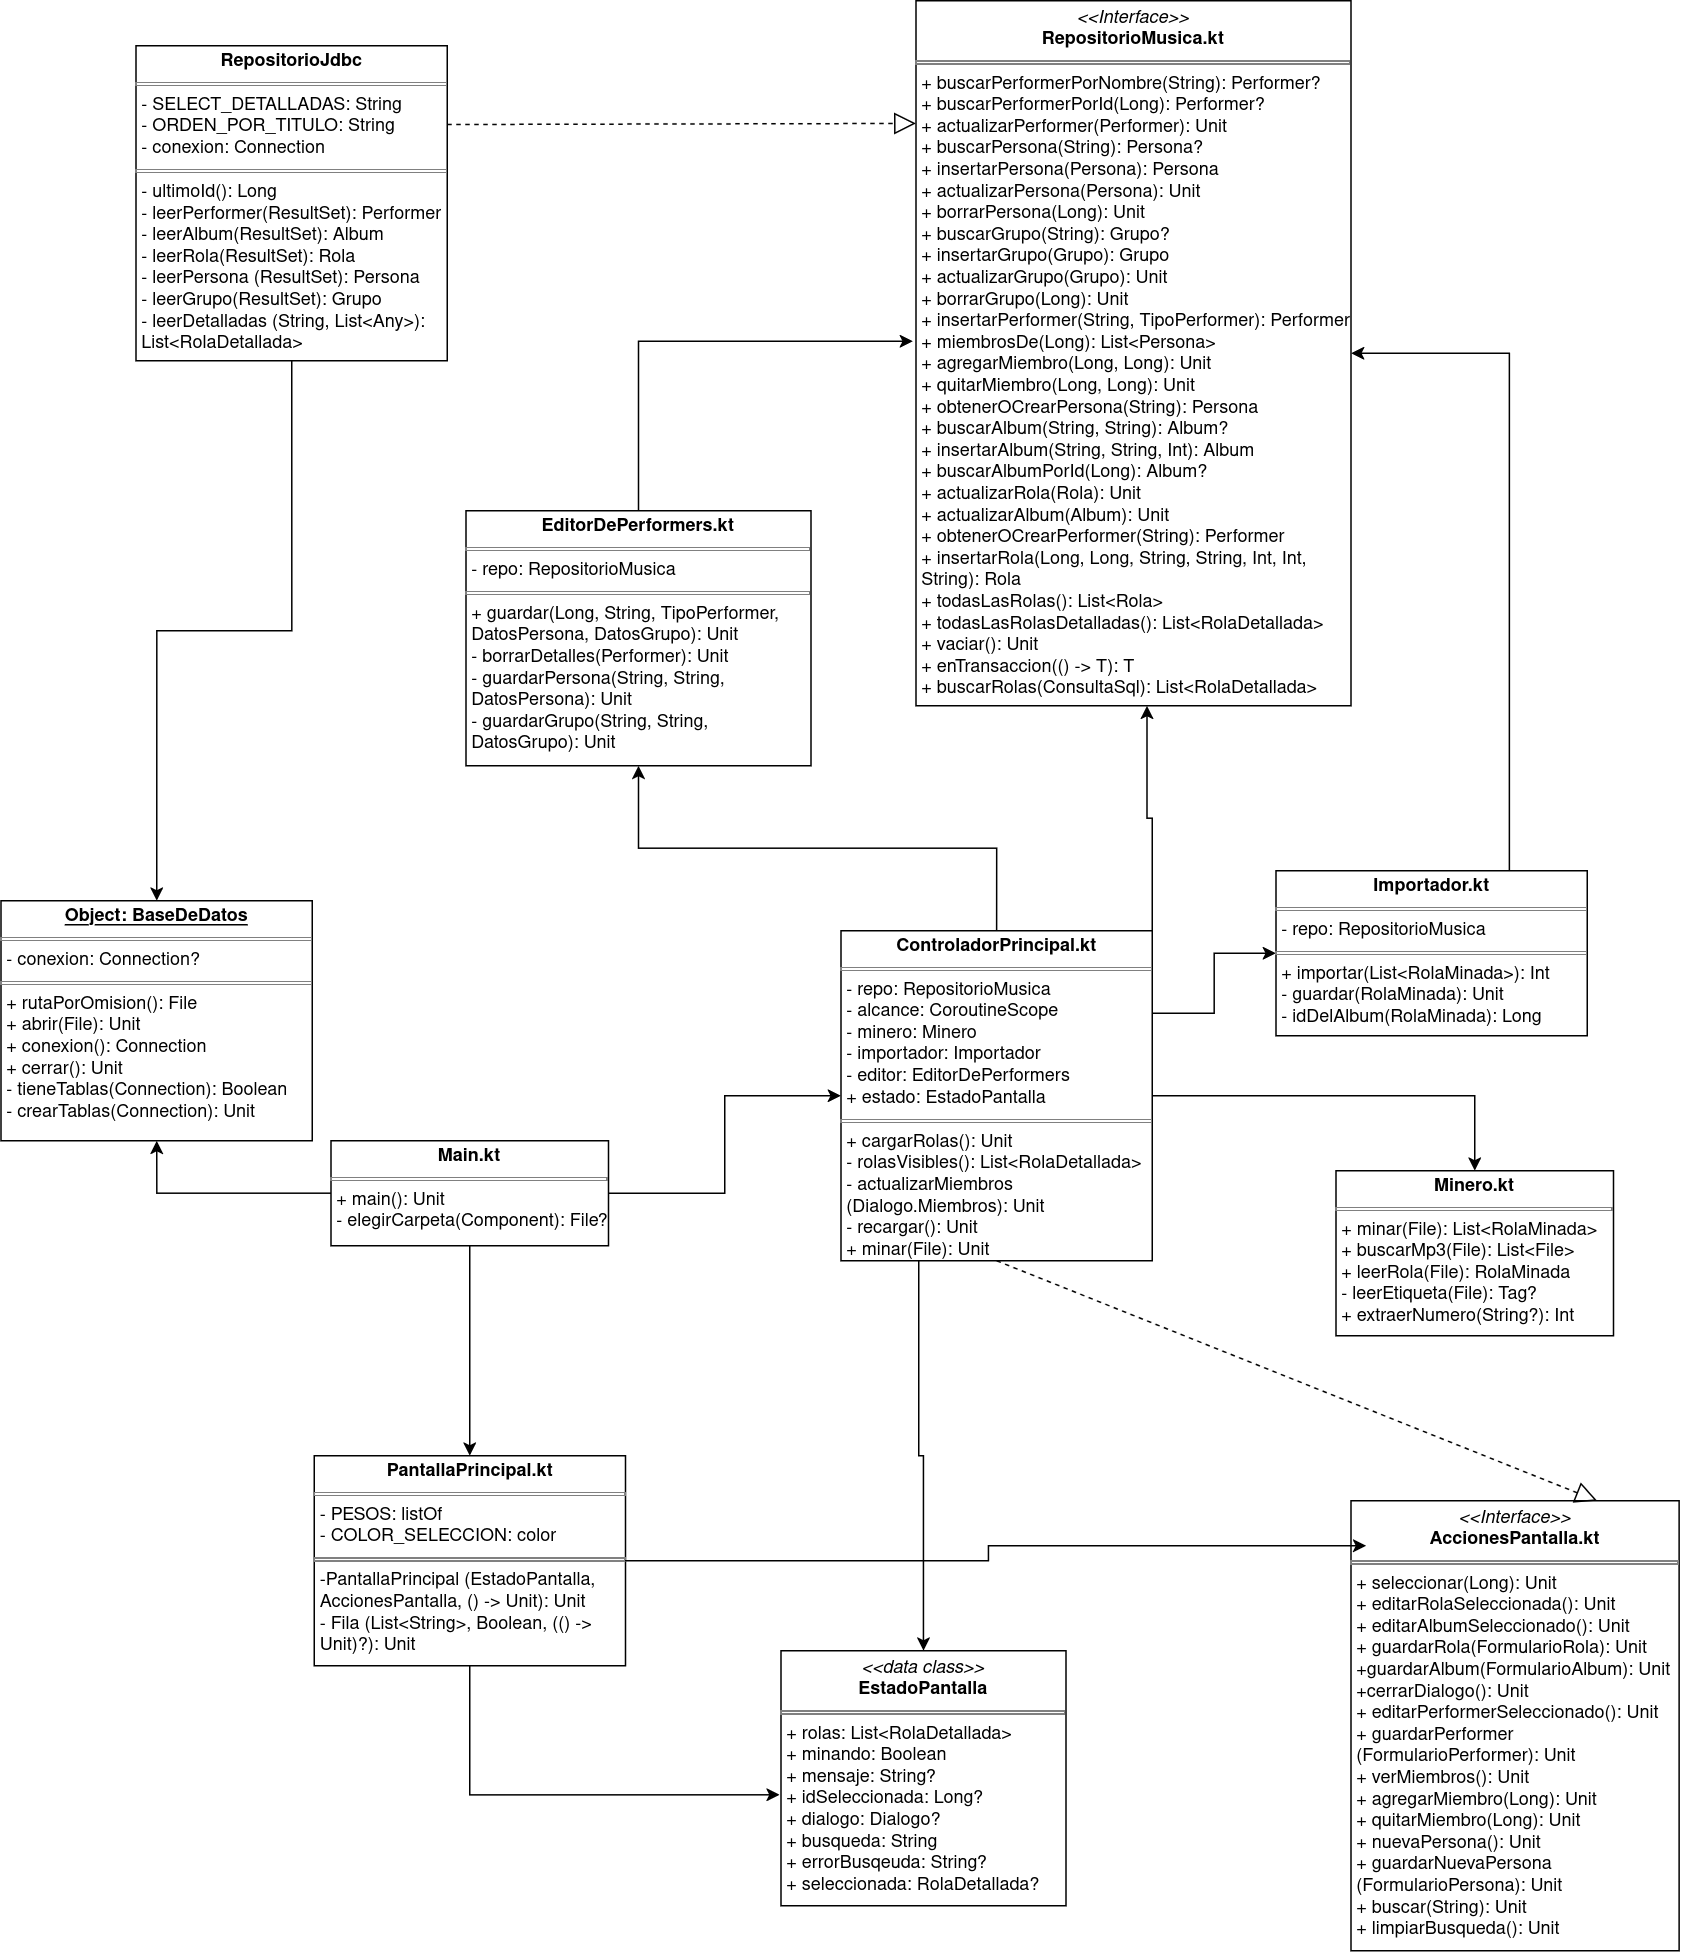
\includegraphics[width=\textwidth, height=0.75\textheight, keepaspectratio]{Diagrama1.drawio.png}
    \caption{Diagrama de clases del programa.}
\end{figure}

\begin{figure}[H]
    \centering
    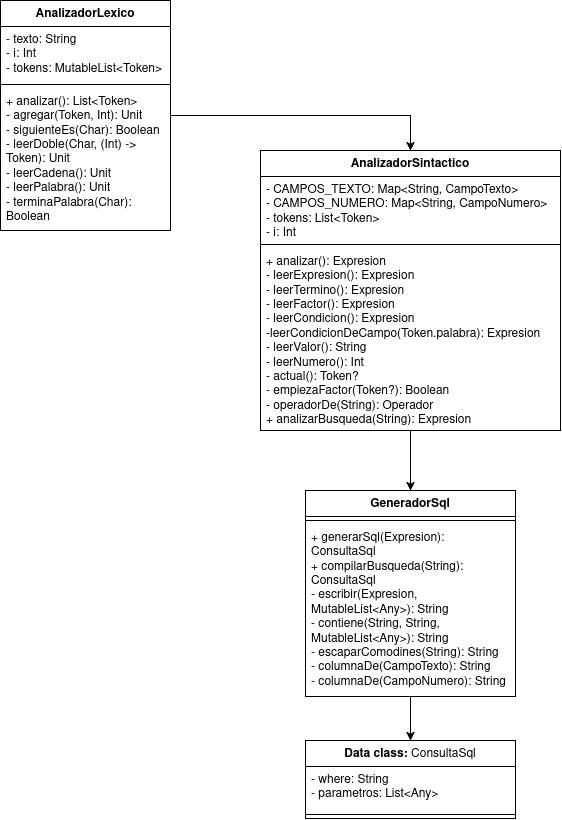
\includegraphics[width=0.8\textwidth, height=0.75\textheight, keepaspectratio]{Diagrama2.drawio.png}
    \caption{Diagrama del compilador.}
\end{figure}
\clearpage

\section{Implementación}

\subsection{Tecnologías utilizadas}

Para este proyecto utilicé Kotlin, porque ya lo conocía del proyecto
anterior y porque tenía planeado que el programa funcionara tanto en
computadora como en Android. Para la interfaz utilicé Kotlin
Multiplatform y Compose Multiplatform, y por eso el código se divide en
dos partes: \texttt{commonMain}, con el código que serviría en cualquier
plataforma, y \texttt{jvmMain}, con lo exclusivo de la computadora. Por la
misma razón utilicé Gradle en lugar de Maven, ya que Compose lo necesita,
a pesar de que yo estaba más familiarizado con Maven.

Para la base de datos utilicé SQLite con el driver sqlite-jdbc, que ya
trae el motor de SQLite incluido, así que no hay que instalar nada aparte;
el programa le manda las instrucciones de SQL a través de JDBC. Para leer
las etiquetas ID3v2.4 de los archivos MP3, que fue una parte crucial del
programa, utilicé la biblioteca jaudiotagger. También utilicé las
corrutinas de Kotlin, para que la ventana no se congele mientras se mina
una carpeta o se hace alguna otra tarea que tarde. Por último, utilicé
kotlin.test para las pruebas unitarias.

\subsection{Arquitectura usada}

Organicé el proyecto con el patrón Modelo-Vista-Controlador, dividido de
la siguiente manera:

\begin{itemize}
    \item \textbf{Modelo}: las clases de datos (\texttt{Rola},
          \texttt{Album}, \texttt{Performer}, \texttt{Persona} y
          \texttt{Grupo}), la base de datos (\texttt{BaseDeDatos},
          \texttt{RepositorioMusica}, \texttt{RepositorioJdbc} y
          \texttt{EditorDePerformers}), el minero (\texttt{Minero} e
          \texttt{Importador}) y el compilador.
    \item \textbf{Vista}: \texttt{PantallaPrincipal},
          \texttt{PanelLateral}, los diálogos y la barra de búsqueda.
          Estas clases no tienen lógica: solo dibujan lo que se les da y
          avisan cuando el usuario hace algo.
    \item \textbf{Controlador}: \texttt{ControladorPrincipal}, que recibe
          lo que hace el usuario, le pide el trabajo al modelo y actualiza
          un \texttt{EstadoPantalla}, que es como una foto de lo que la
          vista debe mostrar. Cuando el estado cambia, Compose vuelve a
          dibujar la pantalla por sí solo.
\end{itemize}

En el proyecto anterior, el del chat, hice una interfaz
\texttt{UsuarioConectado} para que el modelo no dependiera del
controlador. Aquí utilicé la misma idea en dos lugares:

\begin{itemize}
    \item \texttt{RepositorioMusica}: el resto del programa solo conoce
          \emph{qué} se puede hacer con la base de datos, pero no
          \emph{cómo} se hace (con JDBC). Para llevar el proyecto a
          Android bastaría con escribir otra implementación de esta
          interfaz.
    \item \texttt{AccionesPantalla}: la vista solo conoce el ``menú'' de
          acciones que puede pedir, y no al controlador real.
\end{itemize}


\subsection{El patrón Singleton}

Para la base de datos utilicé el patrón de diseño Singleton. La clase
\texttt{BaseDeDatos} es un \texttt{object} de Kotlin, lo que garantiza que
solo existe una instancia de ella y, por lo tanto, una sola conexión a la
base de datos, compartida por todo el programa. Al abrirla, si la base
todavía no tiene las tablas, se crea el esquema que nos proporcionó el
profesor, y además se activan las llaves foráneas, que SQLite trae
desactivadas por defecto.

\begin{verbatim}
object BaseDeDatos {
    private var conexion: Connection? = null

    fun abrir(archivo: File = rutaPorOmision()) { ... }

    fun conexion(): Connection =
        conexion ?: throw IllegalStateException("La base de datos no está abierta")
}
\end{verbatim}

Tener una sola conexión es importante por las transacciones: una
transacción pertenece a una conexión, así que si el minero usara una
conexión y el importador otra, las rolas insertadas por uno no formarían
parte de la transacción del otro, y el ``todo o nada'' dejaría de
funcionar. Además, \texttt{BaseDeDatos} recibe la ruta del archivo al
abrirse: el programa usa siempre la misma, mientras que las pruebas usan
una base temporal, para no modificar la biblioteca real del usuario.

\subsection{Transacciones}

Una transacción agrupa varias operaciones en una sola, de modo que o se
guardan todas, o no se guarda ninguna. En el programa esto se hace con
\texttt{enTransaccion \{ ... \}}: si las operaciones del bloque terminan
bien, se guardan con \texttt{commit()}; si algo sale mal, se deshacen
todas con \texttt{rollback()}.

\begin{verbatim}
fun importar(rolas: List<RolaMinada>): Int =
    repo.enTransaccion {
        repo.vaciar()
        for (rola in rolas) guardar(rola)
        rolas.size
    }
\end{verbatim}

Las transacciones se utilizan, por ejemplo, en el re-minado, donde vaciar
la base y volver a insertar todas las canciones va en una sola
transacción. Si el minado falla a la mitad, la biblioteca anterior queda
intacta. Además, hace que el minado sea mucho más rápido, porque sin una
transacción SQLite guardaría en el disco después de cada rola, mientras
que con ella lo guarda todo de una sola vez al final. También se utilizan
al editar un intérprete: si el nombre nuevo ya lo tiene otro, se deshace
todo lo que ya se había cambiado.

Un caso especial son las transacciones anidadas. La función
\texttt{importar} abre una transacción y, dentro de ella, llama a
\texttt{vaciar}, que a su vez abre otra. Para que no choquen, si ya hay
una transacción abierta, la de adentro solo ejecuta su bloque y deja que
la de afuera decida si se guarda todo o se deshace.

\subsection{El compilador}

El compilador toma lo que escribe el usuario en el lenguaje sencillo del
buscador y lo convierte en SQL. Consta de tres etapas:

\begin{enumerate}
    \item \textbf{Analizador léxico.} Recorre el texto letra por letra y
          lo corta en piezas llamadas \emph{tokens}: palabras, textos
          entre comillas, dos puntos, comparadores, los operadores
          \texttt{y}, \texttt{o} y \texttt{no}, y paréntesis. En esta
          etapa, las palabras \texttt{y}, \texttt{o} y \texttt{no} se
          reconocen como operadores, y un texto entre comillas, como
          \texttt{"texto y más texto"}, se lee completo como una sola
          pieza.
    \item \textbf{Analizador sintáctico.} Acomoda los tokens en un árbol.
          Para esto se usa la técnica de \emph{descenso recursivo}, que
          consiste en escribir una función por cada regla de la
          gramática: \texttt{leerExpresion} para el operador O,
          \texttt{leerTermino} para Y, y \texttt{leerFactor} para NO y
          los paréntesis. El orden en el que se resuelven los operadores
          (primero \texttt{no}, luego \texttt{y} y al final \texttt{o})
          sale solo de qué función llama a cuál, y los paréntesis
          funcionan porque \texttt{leerFactor} vuelve a llamar a
          \texttt{leerExpresion} para leer lo que hay dentro de ellos.
    \item \textbf{Generador.} Recorre el árbol y escribe la parte
          \texttt{WHERE} de la consulta, con un \texttt{?} en el lugar de
          cada valor, y la lista de esos valores por separado.
\end{enumerate}

La gramática que sigue el analizador sintáctico es la siguiente:

\begin{verbatim}
expresion := termino ( O termino )*
termino   := factor ( Y factor )*
factor    := NO factor | ( expresion ) | condicion
condicion := campo : valor | campo comparador numero | valor
\end{verbatim}

\subsection{Validación y manejo de errores}

\textbf{Formularios.} Lo que escribe el usuario en un diálogo siempre es
texto. Por eso, primero se valida que no esté vacío, que los números sean
números y que las fechas existan, incluidos los años bisiestos, y solo
entonces se convierte y se guarda. Si algo está mal, el diálogo muestra el
error.

\textbf{Excepciones propias.} \texttt{NombreRepetidoException} se lanza
cuando se intenta ponerle a un intérprete el nombre de otro, y
\texttt{ErrorDeSintaxis} cuando una búsqueda está mal escrita, junto con
un mensaje que dice qué falló y en qué posición.

\textbf{Sentencias preparadas.} Los valores nunca se pegan directamente en
el texto del SQL. En su lugar, la consulta se escribe con huecos
(\texttt{?}) y los valores se mandan por separado, de modo que SQLite
nunca confunde un valor con una instrucción. Esto evita varios problemas.
Por ejemplo, un título con apóstrofo, como \texttt{'Ach, Ich Fühl's},
rompería la consulta si se pegara tal cual. También protege contra la
\emph{inyección SQL}: si alguien busca \texttt{titulo: "x' OR '1'='1"}
intentando que la condición siempre sea verdadera y aparezcan todas las
rolas, ese texto se trata como un título a buscar, así que solo aparecería
una rola cuyo título lo contenga literalmente.

\textbf{Comodines.} En SQL, la búsqueda por ``contiene'' usa caracteres
especiales llamados comodines: \texttt{\%} significa ``cualquier cantidad
de letras'' y \texttt{\_} significa ``una sola letra''. Si el usuario
escribe uno de estos caracteres, por ejemplo al buscar
\texttt{titulo: 100\%}, se busca el carácter de verdad y no se usa como
comodín.

\subsection{Pruebas}

Cada prueba que utiliza la base de datos crea una base temporal nueva y la
borra al terminar. Así, las pruebas no se estorban entre sí y nunca se
toca la base de datos real. Se hicieron pruebas para el minero, el
repositorio, el importador, el editor de intérpretes, cada etapa del
compilador, la búsqueda completa contra una base con rolas, la validación
de los formularios y el controlador. Gracias a MVC, el modelo se pudo
probar sin abrir la ventana.

Algo que me pasó varias veces fue que, al agregar un tipo de diálogo
nuevo, el proyecto dejaba de compilar y no podía correr ni las pruebas.
Me costó entender por qué, hasta que vi que el \texttt{when} que decide
qué diálogo dibujar no tenía el caso nuevo. Como los diálogos están
definidos con un \texttt{sealed interface}, Kotlin obliga a cubrir todos
los casos, así que en lugar de que se me olvidara dibujar un diálogo y lo
descubriera hasta usar el programa, el compilador me avisó desde antes.

Otro error que encontraron las pruebas fue un espacio que faltaba en una
consulta de SQL escrita en dos líneas: las palabras quedaban pegadas y
SQLite no entendía la consulta. Fallaron tres pruebas a la vez, y lo que
tenían en común me llevó directo a la función con el error.

\subsection{Compilación y uso}

Para compilar y ejecutar el programa solo se necesita tener Java
instalado, porque Gradle descarga lo demás. Desde la carpeta del
proyecto, el programa se ejecuta con:

\begin{verbatim}
$ ./gradlew :desktopApp:run
\end{verbatim}

y las pruebas se corren con:

\begin{verbatim}
$ ./gradlew :shared:jvmTest
\end{verbatim}

La base de datos se guarda en
\texttt{\textasciitilde/.local/share/music-kotlin/musica.db}, así que las
rolas siguen ahí la próxima vez que se abra el programa.

Para usarlo, el usuario presiona ``Minar carpeta'' y escoge la carpeta con
su música. Al terminar aparecen todas las rolas en la lista; al hacer clic
en una, sus datos se muestran en el panel de la izquierda, donde con
``Editar'' se pueden modificar la rola, su intérprete o su álbum. Con
``Nueva persona'' se dan de alta personas, y desde la edición de un grupo
se agregan sus miembros. Para buscar, el usuario escribe en la barra de
búsqueda y presiona Enter, por ejemplo:

\begin{itemize}
    \item \texttt{malilla}
    \item \texttt{interprete: "charle ans"}
    \item \texttt{genero: rap o genero: jazz}
    \item \texttt{interprete: malilla y año > 2020}
\end{itemize}

y con ``Limpiar'' vuelve a ver todas las rolas.

\section{Conclusiones}

En conclusión, este proyecto fue muy desafiante, ya que utilicé muchas
cosas completamente nuevas, aunque ya tenía una idea de cómo funcionaban o
de cómo se podían hacer. Comparado con el proyecto anterior, sin duda fue
más difícil: tuve que aprender a usar Gradle; hacer una interfaz gráfica
desde cero, que, aunque ya había visto una en ICC, fue algo tedioso;
entender la base de datos y cómo se relacionan sus tablas, que fue
bastante laborioso; investigar qué biblioteca utilizar en el minero para
leer las etiquetas, y construir el compilador, que fue sin duda uno de los
mayores retos.

Mi aprendizaje más grande fue la base de datos: los JOIN, las
transacciones y ver cómo se enlaza cada tabla con las demás, sobre todo
porque el esquema no se podía modificar y tuve que resolver cómo conectar
a los intérpretes con sus personas y sus grupos. También aprendí a usar el
patrón Singleton para que todo el programa compartiera una sola conexión,
y a separar el código para que solo el repositorio escribiera SQL, en
lugar de que cualquier parte del programa pudiera modificar la base de
datos.

Las pruebas, igual que en el proyecto anterior, fueron fundamentales. Me
ayudaron a encontrar errores que a simple vista no se notaban, como un
espacio que faltaba en una consulta de SQL, y me daban la confianza de
que, al agregar algo nuevo, lo que ya funcionaba no se rompía. Además,
gracias al patrón Modelo-Vista-Controlador pude probar toda la lógica del
programa sin tener que abrir la ventana ni hacer clic en nada, y entendí
mejor por qué es importante que el modelo no dependa de la vista ni del
controlador.

En el futuro me gustaría mejorar varias cosas: que se pueda reproducir la
música, que aparezca un disco de vinilo con la portada de cada canción,
que la búsqueda también ignore las mayúsculas en las letras con acento y,
algo que estaría genial, terminar la versión para Android.

Este proyecto de verdad me gustó, porque me desafió con todo lo que tenía.
A pesar de que lo empecé lo más rápido posible, casi no me alcanzó el
tiempo para terminarlo, y eso me hizo ver todo el trabajo que hay detrás
de aplicaciones que usamos todos los días, como Spotify. Me gustaría
seguir actualizándolo como un proyecto personal. Además, gracias a él
resolví una duda que tenía desde hace años: por qué, en mi época de
secundaria, cuando escuchaba música en Play Música, algunos artistas o
álbumes aparecían como ``Unknown''.

\section{Bibliografía}

\begin{itemize}
    \item Documentación de Kotlin: \url{https://kotlinlang.org/docs/home.html}
    \item Corrutinas de Kotlin: \url{https://kotlinlang.org/docs/coroutines-overview.html}
    \item Compose Multiplatform: \url{https://www.jetbrains.com/help/kotlin-multiplatform-dev/compose-multiplatform-create-first-app.html}
    \item Documentación de Gradle: \url{https://docs.gradle.org/}
    \item Documentación de SQLite: \url{https://www.sqlite.org/docs.html}
    \item SQLite, transacciones: \url{https://www.sqlite.org/lang_transaction.html}
    \item SQLite, llaves foráneas: \url{https://www.sqlite.org/foreignkeys.html}
    \item SQLite, expresiones y \texttt{LIKE}: \url{https://www.sqlite.org/lang_expr.html}
    \item sqlite-jdbc: \url{https://github.com/xerial/sqlite-jdbc}
    \item Sentencias preparadas en JDBC: \url{https://docs.oracle.com/javase/tutorial/jdbc/basics/prepared.html}
    \item jaudiotagger: \url{https://bitbucket.org/ijabz/jaudiotagger}
    \item Patrón Singleton: \url{https://refactoring.guru/es/design-patterns/singleton}
\end{itemize}

\end{document}
